\documentclass{beamer}
\usefonttheme{professionalfonts}
\usetheme[subsectionpage=progressbar]{metropolis}
\setbeamertemplate{section in toc}[sections numbered]
\setbeamertemplate{subsection in toc}[subsections numbered]

\title{Riemannian Symmetric Rank One Trust Region Method}
\subtitle{in \lstinline!Manopt.jl!}
\author{Tom-Christian Riemer}
\institute{TU Chemnitz}
\date{Research Seminar Numeric,\\ 9th Juny 2021}

%packages
\usepackage{amsmath}
\usepackage[british]{babel}
\usepackage[utf8]{inputenc}
\usepackage{enumerate}
\usepackage{graphicx}
\usepackage{mathtools}
\usepackage{color}
\usepackage{listings}
\usepackage[]{algorithm2e}

\lstset{basicstyle=\ttfamily,	tabsize=2}

\newcommand\myeq{\stackrel{\mathclap{\mbox{$def$}}}{=}}

\newcommand{\Pb}[1]{\expandafter\hat#1}

\begin{document}

\maketitle

\begin{frame}{Contents}
	\tableofcontents
\end{frame}

\section{Introduction}

\begin{frame}{Riemannian Optimization}
    Finding a \textbf{minimum} of a real-valued function $f$ on a Riemannian manifold, i.e.
    \begin{equation*}
        \min f(x), \quad x \in \mathcal{M}.
    \end{equation*}\\[1.\baselineskip]
    \begin{center}
        \textbf{Riemannian manifold} = smooth manifold + Riemannian metric. \\[1.\baselineskip]
    \end{center}
    \begin{equation*}
        \mathbb{S}^{n-1} = \{ x \in \mathbb{R}^n \colon \; \lVert x \rVert_2 = 1 \}.
    \end{equation*}
\end{frame}

\begin{frame}{Euclidean Trust Region Method}
    
\end{frame}

\begin{frame}{Riemannian Metric and Tangent Spaces}
    
\end{frame}

\begin{frame}{Retractions}
    \vspace{-1\baselineskip}\hfill{\tiny{[Bergmann, 2017]}}
    \begin{center}
        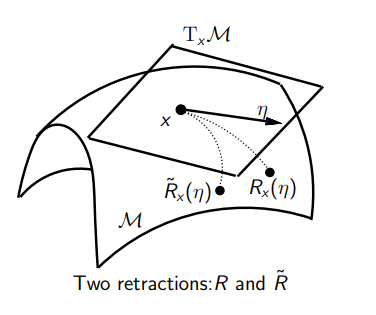
\includegraphics[width=4.5cm]{img/Retraction.png}
    \end{center}
    \textbf{Retraction} $R_{x}(\xi_x) \in \mathcal{M}$ with $R_x (0_x) = x$ and $\mathrm{D} \, R_x (0_x)[\xi_x] = \xi_x$.
\end{frame}

\section{Numerics}

\begin{frame}{Rayleigh Quotient Minimization}
    $A \in \mathbb{R}^{n \times n}$ symmetric, the unit-norm eigenvector, $v \in \mathbb{R}^n$, corresponding to the smallest eigenvalue, defines the two global minima, $\pm v$, of the Rayleigh quotient  
    \begin{equation*}
        \begin{split}
            f \colon \; \mathbb{S}^{n-1} & \to \mathbb{R} \\
            x & \mapsto x^{\mathrm{T}} A x 
        \end{split}
    \end{equation*}   
    with its Riemannian gradient \\[.3\baselineskip]
    \begin{equation*}
        \operatorname{grad} f(x) = 2(Ax - x x^{\mathrm{T}} A x).
    \end{equation*}
\end{frame}

\begin{frame}{Experiment}
    Julia Code
\end{frame}

\begin{frame}{Results}
    Table with results.
\end{frame}

\section{Conclusion}

\begin{frame}{Conclusion}
    
    \begin{center}
        Thank you for your attention! Questions? 
    \end{center}
\end{frame}

\end{document}
